\label {fs-short-experiments}

\begin{figure*}[t!]
    \begin{subfigure}[b]{0.31\textwidth}
            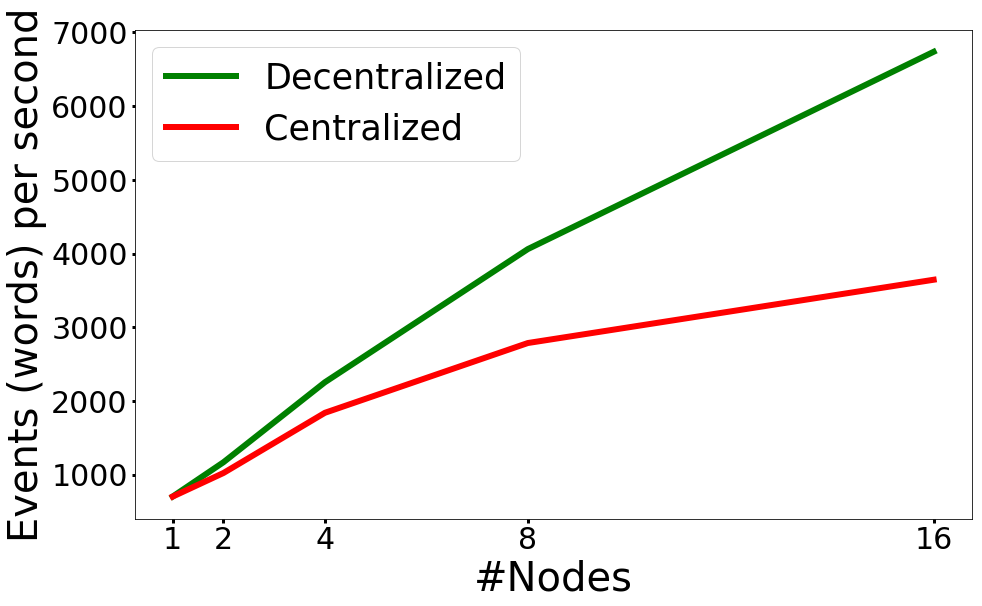
\includegraphics[width=\linewidth]{pics/throughput}
            \caption{Throughput for centralized and decentralized approaches}
            \label{throughput}
    \end{subfigure}%
    \hspace{5mm}
    \begin{subfigure}[b]{0.31\textwidth}
            \includegraphics[width=\linewidth]{pics/detection_rate}
            \caption{Change detection speed for round robin and hash partitionings}
            \label{detection_rate}
    \end{subfigure}%
    \hspace{5mm}
    \begin{subfigure}[b]{0.31\textwidth}
            \includegraphics[width=\linewidth]{pics/decision_making.png}
            \caption{A comparison between decision making approaches}
            \label{decision_making}
    \end{subfigure}%
    \caption{Results of preliminary experiments}
\end{figure*}


\indent

{\bf Setup.} We conducted several experiments to evaluate if the proposed problem statement is reasonable. We used words from Wikipedia corpus as an input stream for experiments. Such stream of words can be considered as a part of word count or IDF computing pipelines. A validation task is to check that frequencies of input words fit Zipf distribution. As it was mentioned above, this validation task is useful for fraud detection.

{\bf Throughput.} We measured throughput of two approaches: centralized, where words are merged to a single node for validation, and decentralized. Experiments were conducted with Apache Flink on a cluster of Amazon EC2 small instances with 1 core CPU and 2GB RAM. Figure~\ref{throughput} shows that centralized method significantly limits throughput and scalability of the whole data flow. This result demonstrates that proposed problem statement has practical rationale.

{\bf Change detection speed.} In this experiment we measure the duration (in input events) of change detection. A change in data is simulated using input from generated corpus with lognormally distributed word frequencies. We compared two data partitioning methods. The first one is natural for word count and IDF computing task: each word sticks to a concrete node. In this case, each node processes only its own subsample of all possible words. The second approach is round robin. While it is not suitable for word count, such partitioning ensures that each word may be processed on all computational nodes. As expected, Figure~\ref{detection_rate} demonstrates that round robin provides faster detection, because simulated lognormal data is distributed among nodes in a more uniform way. This behavior means that for faster detection, it may be reasonable to reshuffle words in a round-robin manner after, e.g. IDF aggregation.

{\bf Making decisions approaches.} This experiment demonstrates comparison between three simple mechanisms for making a global decision about hypothesis acceptance based on local decisions of each node. The first method indicates that hypothesis is rejected if at least one node rejects it. The second technique make the decision based on a majority vote of all nodes decisions. Last method rejects hypothesis only if all nodes rejects it. Figure~\ref{decision_making} shows a dependency between number of nodes and number of input elements needed to detect change for round robin partitioning. As we can see, method that   